% -----------------------------------------------------------------------------
% Project: PhD KAPPA
% File: kappa.Rnw (root file)
% Author: Alessio Crippa
% Template: based on the tex code written by Andrea Discacciati
%           url: https://github.com/anddis/phd-thesis
%
% Purpose: Root Rnw file, compile this to typeset the kappa!
% -----------------------------------------------------------------------------



% If you get the following error:
%  Error in ensurePackageSymlink(source, target) :
% run the next line, an then restart your R session
% unlink("packrat/lib-R", recursive = TRUE)


% Class
\documentclass[11pt,a4paper,twoside,openany]{book}\usepackage{knitr}

% Packages
\usepackage[english]{babel}
\usepackage{amsfonts}
\usepackage{amsmath}
\usepackage{mathtools}
\usepackage{threeparttable}
\usepackage{adjustbox}
\usepackage{natbib}
\usepackage{graphicx}
\usepackage{flafter}
\usepackage{fancyhdr}
\usepackage{textcomp}
\usepackage[utf8]{inputenc}
\usepackage{setspace}
\usepackage[pdftex,
            pdfauthor={Alessio Crippa},
            pdftitle={Novel methods for dose--response meta-analysis},
            pdfcreator={LaTeX2e}]{hyperref}
\usepackage[%showframe,
			headheight=13.6pt,
			%headsep=,
			%footskip=,
			bindingoffset=0cm,%print=.5cm, web=0cm
			left=3cm,  %print=2cm, web=3cm
			bottom=3cm, %print=3cm, web=3cm
			top=3cm, %print=3cm, web=3cm,
			right=3cm]{geometry} %print=3.5cm, web=3cm
\usepackage{enumerate, mdwlist}
\usepackage{etoolbox}
\usepackage{tabularx}
\usepackage{rotating}
\usepackage[font={small}]{caption}
\usepackage{chngcntr}
\counterwithout{footnote}{chapter}

%---begin see http://www.khirevich.com/latex/font/
\usepackage[activate={true,nocompatibility},final,tracking=true,kerning=true,spacing=true,factor=1100, stretch=10,shrink=10]{microtype}
% remove warning
\microtypecontext{spacing = nonfrench}
\usepackage[T1]{fontenc}
% remove warning
\global\expandafter\let\csname ver@amsfonts.sty\endcsname\relax
% remove issue related to interwordspace
\setlength{\emergencystretch}{10pt}
\usepackage[bitstream-charter]{mathdesign}
\usepackage{sectsty}
	\chapterfont{\usefont{T1}{qhv}{b}{n}\selectfont\huge}
\usepackage{titlesec}

% ---------------------------------------------------------
% Project: PhD KAPPA
% File: _titlesec.tex
% Author: Andrea Discacciati
%
% Purpose: Headings format
%			(see titlesec package)
% ---------------------------------------------------------

\titleformat{\section}[hang]{
    \usefont{OT1}{qhv}{bx}{n}\selectfont}
    {} 
    {0em}
    {\hspace{-0.4pt}\Large \thesection\hspace{0.6em}}
\titleformat{\subsection}[hang]{
    \usefont{OT1}{qhv}{bx}{n}\selectfont}
    {} 
    {0em}
    {\hspace{-4pt} \thesubsection\hspace{0.6em}}
\titleformat{\subsubsection}[hang]{
    \usefont{OT1}{qhv}{bx}{n}\selectfont}
    {} 
    {0em}
    {\normalsize}
\usepackage{tocloft}

% ---------------------------------------------------------
% Project: PhD KAPPA
% File: _tocloft.tex
% Author: Andrea Discacciati
%
% Purpose: Table of Contents, 
%			List of Figures, List of Tables format
%			(see tocloft package)
% ---------------------------------------------------------

\renewcommand{\cfttoctitlefont} % ToC title
             {\usefont{T1}{qhv}{b}{n}\selectfont\huge}
\renewcommand{\cftchapfont} % chapter titles
             {\usefont{T1}{qhv}{b}{n}\selectfont}
\renewcommand{\cftsecfont} % section titles
             {\usefont{T1}{bch}{m}{n}\selectfont}
\renewcommand{\cftsubsecfont} % subsection titles
             {\usefont{T1}{bch}{m}{n}\selectfont} 
\renewcommand{\cftchappagefont} % chapter page numbers
             {\usefont{T1}{bch}{b}{n}\selectfont}
\renewcommand{\cftsecpagefont} % section page numbers
             {\cftsecfont} 
\renewcommand{\cftsubsecpagefont} % subsection page numbers
             {\cftsubsecfont}
             
\renewcommand{\cftloftitlefont} % LoF title
             {\usefont{T1}{qhv}{b}{n}\selectfont\huge}
\renewcommand{\cftfigfont} % Figures titles
             {\usefont{T1}{bch}{m}{n}\selectfont}
             
\renewcommand{\cftlottitlefont} % LoT title
             {\usefont{T1}{qhv}{b}{n}\selectfont\huge}
\renewcommand{\cfttabfont} % Tables titles
             {\usefont{T1}{bch}{m}{n}\selectfont}
%---end see http://www.khirevich.com/latex/font/

% Header / footer

% ---------------------------------------------------------
% Project: PhD KAPPA
% File: _fancyhdr.tex
% Author: Alessio Crippa
% based on the template written by Andrea Discacciati
%
% Purpose: Header and footer settings
%			(see fancyhdr package)
% ---------------------------------------------------------

\pagestyle{fancy}
\renewcommand{\chaptermark}[1]{%
 \markboth{{\thechapter.\ #1}}{}}

\fancypagestyle{plain}{%
  \fancyhf{}%
  \renewcommand{\headrulewidth}{0pt}%
  \fancyhf[lef,rof]{}%
  %\fancyhead[LE,RO]{\thepage}
}

\fancypagestyle{frontmatter}{%
  \renewcommand{\headrulewidth}{0pt} 
  \renewcommand{\footrulewidth}{0pt}
  \fancyhf{}% Clear header/footer
  \fancyhead[LE,RO]{}
}

\fancypagestyle{nothing}{%
  \renewcommand{\headrulewidth}{0pt} 
  \renewcommand{\footrulewidth}{0pt}
  \fancyhf{}% Clear header/footer
  \fancyhead[LE,RO]{}%
}

\fancypagestyle{mainmatter}{%
  \renewcommand{\headrulewidth}{.4pt}
  \renewcommand{\footrulewidth}{0pt}
  \fancyhf{}% Clear header/footer
  \fancyhead[LE,RO]{\thepage}
  \fancyhead[RE,LO]{\nouppercase \leftmark}
}

	
% See 'writing a thesis with latex' p25 
% Writes nothing on empty pages
\makeatletter
\def\cleardoublepage{\clearpage\if@twoside
\ifodd\c@page
\else\hbox{}\thispagestyle{empty}\newpage
\if@twocolumn\hbox{}\newpage\fi\fi\fi}
\makeatother

% Substitutions (%examples)
%\newcommand{\rveplot}{decorrelated-residuals--versus--exposure plot}
%\newcommand{\kgmsq}{kg$\times$m\textsuperscript{$-2$}}

\defcitealias{crippadosresmeta2016}{Paper~I}	
\defcitealias{discacciati2015goodness}{Paper~II}	
\defcitealias{crippa2016new}{Paper~III}	
\defcitealias{crippa2018pointwise}{Paper~IV}	
\defcitealias{crippa2018one}{Paper~V}	

%\doublespacing 
\onehalfspacing

\allowdisplaybreaks

\renewcommand{\sfdefault}{qhv}
\newcommand*{\LargerCdot}{\raisebox{-0.25ex}{\scalebox{1.2}{$\cdot$}}}

\DeclareMathOperator{\Cov}{Cov} 
\DeclareMathOperator{\diag}{diag} 
\DeclareMathOperator{\N}{N} 
\DeclareMathOperator{\E}{E}
\DeclareMathOperator{\logit}{logit} 
\DeclareMathOperator{\df}{df} 
\hyphenation{logRRs}
\hyphenation{logRR}

\addto\captionsenglish{%
  \renewcommand{\bibname}{References}%
}

%\includeonly{abstract, results, introduction, background, aims, discussion, conclusions }

%--- Kappa starts here! ---%
\IfFileExists{upquote.sty}{\usepackage{upquote}}{}
\begin{document}

% Front matter
\frontmatter
\pagestyle{nothing}

% ---------------------------------------------------------
% Project: PhD KAPPA
% File: titlepage.tex
% Author: Alessio Crippa
% based on the template written by Andrea Discacciati
%
% Purpose: Custom title page + ISBN/copyright page
% ---------------------------------------------------------

\begin{titlepage}
\newgeometry{margin=4cm}
\begin{center}
\large
From the Department of Public Health Sciences \\
Karolinska Institutet, Stockholm, Sweden        
\vfill
\Large
\textbf{\textsf{NOVEL METHODS FOR DOSE-RESPONSE META-ANALYSIS}}
\vfill
\Large
Alessio Crippa
\vfill

\includegraphics[width=0.8\textwidth]{figures/ki-logo_pos}
\vfill
\large
Stockholm 2018        
\end{center}
\restoregeometry
\end{titlepage}

\newpage
\null
\vfill
\noindent All published papers reproduced with permission \\
%Cover illustration ``Portraits of sophistication'' by Lamai McCartan \\
Published by Karolinska Institutet \\
\bigskip
Printed by E-Print AB 2018 \\
Edited in R using knitr \\
\textcopyright Alessio Crippa, 2018 \\
ISBN <include number>
\newpage

% ---------------------------------------------------------
% Project: PhD KAPPA
% File: spikblad.tex
% Author: Alessio Crippa
% based on the template written by Andrea Discacciati
%
% Purpose: Spikblad
% ---------------------------------------------------------
\null
\vspace{1.5cm}
\noindent{\Large \textsf{NOVEL METHODS FOR DOSE-RESPONSE META-ANALYSIS} \vspace{1cm}}\\
\noindent{\Large \textsf{THESIS FOR DOCTORAL DEGREE (Ph.D.)} \vspace{.5cm}}\\
By \vspace{.5cm} \\
{\Large \textbf{\textsf{Alessio Crippa}} \vspace{2cm}}\\
\begin{minipage}[t]{6.2cm}
\singlespacing
{\small
\textit{Principal supervisor:}\\
Associate Professor Nicola Orsini \\
Karolinska Institutet \\
\bigskip
Department of Public Health Sciences \\
\textit{Co-supervisor:}\\
Professor Alicja Wolk \\
Karolinska Institutet \\
\medskip
Institute of Environmental Medicine \\
Professor Matteo Bottai \\
Karolinska Institutet \\
\medskip
Institute of Environmental Medicine \\
Professor Donna Spiegelman \\
Harvard T.H. Chan School of Public Health \\
Department of Epidemiology
}
\end{minipage}
\hspace{1.5cm}
\begin{minipage}[t]{8.1cm}
\singlespacing
{\small
\textit{Opponent:}\\
Professor Christopher H. Schmid \\
Brown University \\
Center for Evidence Based Medicine\bigskip \\
\textit{Examination board:}\\
Associate Professor Nele Brusselaers \\
Karolinska Institutet \\
Department of Microbiology, Tumor and Cell Biology \medskip \\
Associate Professor Antonio Gasparrini \\
London School of Hygiene and Tropical Medicine \\
Department of Social $\&$ Environmental Health Research\medskip \\
Professor Paul Lambert \\
University of Leicester \\
Department of Health Sciences
}
\end{minipage}
\cleardoublepage

% ---------------------------------------------------------
% Project: PhD KAPPA
% File: dedication.tex
% Author: Alessio Crippa
% based on the template written by Andrea Discacciati
%
% Purpose: Dedication
% ---------------------------------------------------------


\begin{flushright}
\null\vspace{\stretch{1}}
\textit{``If I have seen further, it is by standing on the shoulders of giants.''} \\
---Isaac Newton
\vspace{\stretch{2}}\null
\end{flushright}

\iffalse
\begin{flushright}
\null\vspace{\stretch{1}}
\textit{``This study is really a pile of rubbish, \\ and no one should waste their time reading it.''} \\
---Walter Willett
\vspace{\stretch{2}}\null
\end{flushright}
% http://www.nature.com/news/the-big-fat-truth-1.13039
\fi
\cleardoublepage 
\pagestyle{frontmatter}

% ---------------------------------------------------------
% Project: PhD KAPPA
% File: abstract.tex
% Author: Andrea Discacciati
%
% Purpose: Abstract frontmatter
% ---------------------------------------------------------


\noindent {\Large \textsf{\textbf{{Abstract}}}
\bigskip
%\chapter*{Abstract}
\small
\par My abstract:

In \citetalias{crippadosresmeta2016},

In \citetalias{discacciati2015goodness}, 

In \citetalias{crippa2016new}, 

In \citetalias{crippa2018pointwise},

In \citetalias{crippa2018one},

In conclusion,
\normalsize
\cleardoublepage

% ---------------------------------------------------------
% Project: PhD KAPPA
% File: publications.tex
% Author: Alessio Crippa
% based on the template written by Andrea Discacciati
%
% Purpose: List of publications + related publications
% ---------------------------------------------------------

\chapter*{List of publications}

\begin{enumerate}[I.]
\item Alessio~Crippa, and Nicola~Orsini \\ \textbf{Multivariate dose--response meta-analysis: the dosresmeta R Package} \\ \textit{Journal of Statistical Software, Code Snippets} 2016; 72(1), 1--15
\item Andrea~Discacciati, Alessio~Crippa, and Nicola~Orsini \\ \textbf{Goodness of fit tools for dose--response meta-analysis of binary outcomes} \\ \textit{Research Synthesis Methods} 2015
\item Alessio~Crippa, Polyna~Khudyakov, Molin~Wang, Nicola~Orsini, and Donna~Spiegelman \\ \textbf{A new measure of between-studies heterogeneity in meta-analysis} \\ \textit{Statistics in medicine} 2016; 35(21), 3661--75
\item Alessio~Crippa, Ilias~Thomas, and Nicola~Orsini \\ \textbf{A pointwise approach to dose-response meta-analysis of aggregated data} \\ \textit{Manuscript} 2018
\item Alessio~Crippa, Andrea~Discacciati, Matteo~Bottai, Alicja~Wolk, and Nicola~Orsini \\ \textbf{One-stage dose--response meta-analysis for aggregated data} \\ \textit{Manuscript} 2018
\end{enumerate}
\vspace{1.5cm}
\noindent{The articles will be referred to in the text by their Roman numerals, and are reproduced in full at the end of the thesis.}

\chapter*{Related publications}
\begin{itemize}
\item Alessio~Crippa, Susanna~C.~Larsson, Andrea~Discacciati, Alicja~Wolk, and Nicola~Orsini \\ \textbf{Red and processed meat consumption and risk of bladder cancer: a dose--response meta-analysis of epidemiological studies} \\ \textit{European journal of nutrition} 2016, 1--13
\item Andrea~D.~Smith, Alessio~Crippa, James~Woodcock, and S{\o}ren~Brage \\ \textbf{Physical activity and incident type 2 diabetes mellitus: a systematic review and dose--response meta-analysis of prospective cohort studies} \\ \textit{Diabetologia} 2016, 1--19
\item Marco~Vinceti, Tommaso~Filippini, Alessio~Crippa, Agn{\`e}s~de~Sesmaisons, Lauren~A.~ Wise, and Nicola~Orsini \\ \textbf{Meta-Analysis of Potassium Intake and the Risk of Stroke} \\ \textit{Journal of the American Heart Association} 2016, 5(10), e004210
\item Alessio~Crippa, and Nicola~Orsini \\ \textbf{Dose--response meta-analysis of differences in means} \\ \textit{BMC medical research methodology} 2016, 16(1), 91
\item Emir~Veledar, Alessio~Crippa, Chukwuemeka~U.~Osondu, Adnan~Younus, and Khurram~Nasir \\ \textbf{Letter to Editor: Ideal cardiovascular health metrics and risk of cardiovascular disease or mortality} \\ \textit{International journal of cardiology} 2016, 222, 737
\item Alessio~Crippa, Andrea~Discacciati, Nicola~Orsini, and Viktor~Oskarsson \\ \textbf{Letter: coffee consumption and gallstone disease---a cautionary note on the assignment of exposure values in dose--response meta-analyses} \\ \textit{Alimentary Pharmacology \& Therapeutics} 2016, 43(1), 166-167
\item Susanna~C.~Larsson, Alessio~Crippa, Nicola~Orsini, Alicja~Wolk, and Karl~Micha{\"e}lsson \\ \textbf{Milk consumption and mortality from all causes, cardiovascular disease, and cancer: a systematic review and meta-analysis} \\ \textit{Nutrients} 2016, 7(9), 7749-7763
\item Daniela~Di~Giuseppe, Alessio~Crippa, Nicola~Orsini, and Alicja~Wolk \\ \textbf{Fish consumption and risk of rheumatoid arthritis: a dose-response meta-analysis} \\ \textit{Arthritis research \& therapy} 2014, 16(5), 446
\item Alessio~Crippa, Andrea~Discacciati, Susanna~C.~Larsson, Alicja~Wolk, and Nicola~Orsini \\ \textbf{Coffee consumption and mortality from all causes, cardiovascular disease, and cancer: a dose--response meta-analysis} \\ \textit{American journal of epidemiology} 2014, 180(8), 763-775
\end{itemize}
\cleardoublepage
\microtypesetup{protrusion=false}
\tableofcontents
%\listoffigures
%\newpage
%\listoftables
\microtypesetup{protrusion=true} 

% ---------------------------------------------------------
% Project: PhD KAPPA
% File: abbreviations.tex
% Author: Alessio Crippa
% based on the template written by Andrea Discacciati
%
% Purpose: List of abbreviations
% ---------------------------------------------------------

\chapter*{List of abbreviations}
\begin{tabular}{ll}

AIC & Akaike Information Criterion \\
CI & Confidence Interval \\
df & Degrees of Freedom \\
GLS & Generalized Least Squares \\
GRSS & Generalized Residual Sum of Squares \\
GTSS & Generalized Total Sum of Squares \\
FP2 & Second-degree Fractional Polynomials \\
HRR & Hazard Rate Ratio \\
IR & Incidence Rate \\
IRR & Incidence Rate Ratio \\
logRR & log--Relative Risk \\
MR & Mortality Rate \\
MRR & Mortality Rate Ratio \\
RCS & Restricted Cubic Splines \\
$R^2$ & Coefficient of Determination \\
RR & Relative Risk \\
WLS & Weighted Least Squares


\end{tabular}

% Main matter
\mainmatter
\pagestyle{mainmatter}

% !TeX root = ../kappa.Rnw  


% ---------------------------------------------------------
% Project: PhD KAPPA
% File: introduction.tex
% Author: Andrea Discacciati
%
% Purpose: Introduction
% ---------------------------------------------------------

\chapter{Introduction}

Write my introduction

% !TeX root = ../kappa.Rnw  

% ---------------------------------------------------------
% Project: PhD KAPPA
% File: background.tex
% Author: Alessio Crippa
% based on the template written by Andrea Discacciati
%
% Purpose: Background
% ---------------------------------------------------------

\chapter{Background}

Write my background with subsections.

Here an example of a figure (Figure~\ref{fig:cite_grl}).

\begin{knitrout}
\definecolor{shadecolor}{rgb}{0.969, 0.969, 0.969}\color{fgcolor}\begin{figure}[h]

{\centering 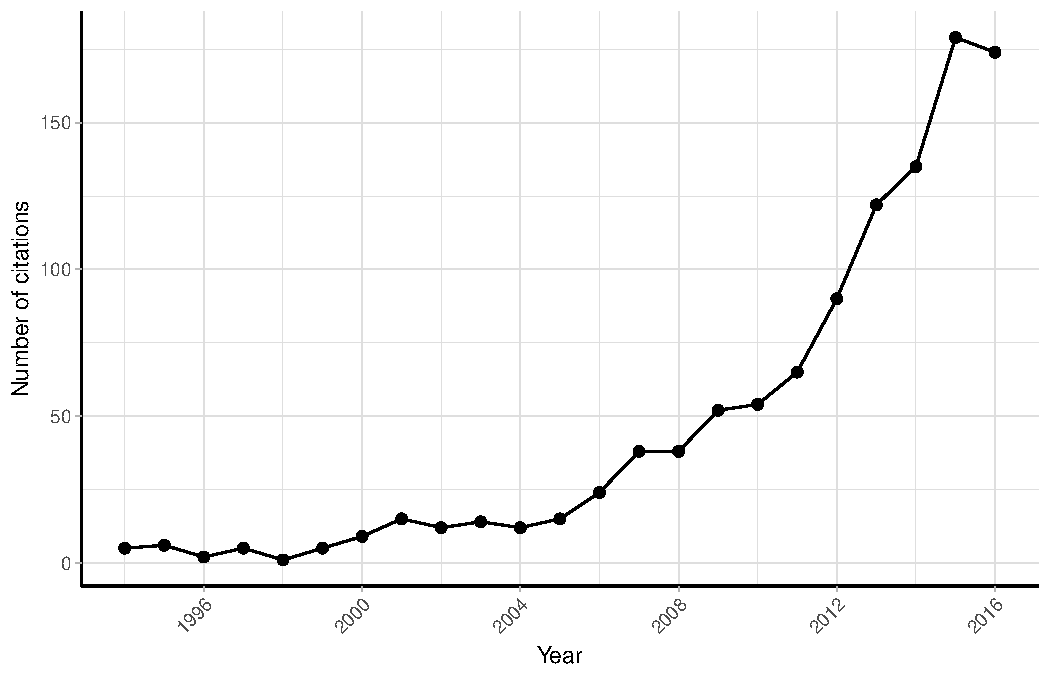
\includegraphics[width=\textwidth]{../figure/cite_grl-1} 

}

\caption[ ]{ }\label{fig:cite_grl}
\end{figure}


\end{knitrout}


% !TeX root = ../kappa.Rnw  


% ---------------------------------------------------------
% Project: PhD KAPPA
% File: aims.tex
% Author: Alessio Crippa
% based on the template written by Andrea Discacciati
%
% Purpose: Aims
% ---------------------------------------------------------

\chapter{Aims of the thesis}

The overall aims of this thesis were to <>.

\bigskip

 More specifically, the aims were:

\begin{itemize}
\item <>

\item <>

\item <>

\item <>
\end{itemize}

% !TeX root = ../kappa.Rnw  


% ---------------------------------------------------------
% Project: PhD KAPPA
% File: materials.tex
% Author: Alessio Crippa
% based on the template written by Andrea Discacciati
%
% Purpose: Materials
% ---------------------------------------------------------

\chapter{Materials and methods}

Write materials and methods with subsections as in the background section

% !TeX root = ../kappa.Rnw  

% ---------------------------------------------------------
% Project: PhD KAPPA
% File: results.tex
% Author: Alessio Crippa
% based on the template written by Andrea Discacciati
%
% Purpose: Results
% ---------------------------------------------------------

\chapter{Results}

Write the results with subsections as in the background section


% Paper I
%\input{results.1}

% !TeX root = ../kappa.Rnw  

% ---------------------------------------------------------
% Project: PhD KAPPA
% File: discussion.tex
% Author: Alessio Crippa
% based on the template written by Andrea Discacciati
%
% Purpose: Discussion
% ---------------------------------------------------------

\chapter{Discussion}

Write the discussion with subsections as in the background section

% !TeX root = ../kappa.Rnw  

% ---------------------------------------------------------
% Project: PhD KAPPA
% File: conclusions.tex
% Author: Alessio Crippa
% based on the template written by Andrea Discacciati
%
% Purpose: Conclusions
% ---------------------------------------------------------

\chapter{Conclusions}

Write summary of conclusions.

More specifically we conclude the following:

\begin{itemize}

\item <>

\item <>

\item <>

\item <> 

\end{itemize}

% !TeX root = ../kappa.Rnw  

% ---------------------------------------------------------
% Project: PhD KAPPA
% File: future.tex
% Author: Alessio Crippa
% based on the template written by Andrea Discacciati
%
% Purpose: Future research
% ---------------------------------------------------------

\chapter{Future research}

Based on the conclusions presented in this thesis, future research includes: 

\begin{itemize}
\item <>

\item <>

\item <>
\end{itemize}

% Appendix
\appendix

% !TeX root = ../kappa.Rnw  

% ---------------------------------------------------------
% Project: PhD KAPPA
% File: appendix.tex
% Author: Alessio Crippa
% based on the template written by Andrea Discacciati
%
% Purpose: Appendix
% ---------------------------------------------------------

\chapter{Supplementary figures}

Figures.

%--tables
\chapter{Supplementary tables}

Tables.

% Back matter
\backmatter
\bibliographystyle{style/jss}
\refstepcounter{chapter}
\addcontentsline{toc}{chapter}{\bibname}
\bibliography{additional/kappa_bib}
\newpage
\pagestyle{nothing}

% ---------------------------------------------------------
% Project: PhD KAPPA
% File: acknowledgements.tex 
% Author: Alessio Crippa
% based on the template written by Andrea Discacciati
%
% Purpose: Acknowledgements
% ---------------------------------------------------------

\chapter{Acknowledgements}

There are many people that I would like to thank for their contributions to this thesis, and for their support and encouragement during these years.

\bigskip

\textbf{Nicola Orsini}, my main supervisor for the second half of my doctoral education.

\bigskip

\noindent This work was supported by \textbf{Karolinska Institutet}'s funding for doctoral students (KID-funding).







\end{document}
